% Chapter 05 - CPET, comorbidity and survival

\chapter{An investigation into the relationship between cardiopulmonary exercise testing, comorbidity, systemic inflammation and survival after pancreaticoduodenectomy for pancreatic ductal adenocarcinoma.}
\label{ch_survival}

\lhead{Chapter \ref{ch_survival}. \emph{CPET, Complications and Survival}} % This is for the header on each page - perhaps a shortened title

\clearpage
%----------------------------------------------------------------------------------------

\section{Introduction}
Median survival after pancreaticoduodenectomy for pancreatic ductal adenocarcinoma varies from approximately 18 months to 24 months.\parencite{winter_1423_2006,neoptolemos_adjuvant_2010} 

Selecting patients who will benefit from the survival advantage that a pancreaticoduodnectomy offers is important to maximise the usefulness of this morbid procedure.

Comorbidity is not only associated with postoperative morbidity and mortality (Section \ref{sec:comorbidity_risk_stratification}) but has also been reported to be associated with poor long-term survival in patients undergoing surgery for several different cancers including colorectal cancer \parencite{} and breast cancer.\parencite{} With 10-year survival rates approaching 60\% and 80\% respectively in patients with these cancers, it is not surprising that some patients with significant comorbidity die of their comorbid disease rather than from cancer recurrence. However, reports suggest that cancer-specific survival is also shorter in patients with significant comorbidities.

Systemic inflammation has been proposed as one of the intermediary mechanism in these patients that increases rates of recurrence and decreases disease free survival. The modified Glasgow Prognostic Score, a measure of preoperative systemic inflammation in cancer patients, is associated with poor survival regardless of the site or stage of cancer. This is discussed in detail in Section \ref{sec:intro_systemic_inflammation_outcome}. 

However, an objective method to measure comorbidity itself remains elusive and various scores have been used for this purpose. The Charlson Comorbidity Index is one such score and has been reported to predict long-term survival in cancer patients. Cardiopulmonary exercise testing is an objective measure of aerobic fitness and of cardiorespiratory comorbidity and has been shown to be useful in predicting complications after major abdominal surgery including pancreatic surgery. (\parencite{ausania_effects_2012} and Chapter \ref{ch_cpet_outcomes})

Moreover, cardiopulmonary exercise testing has been used to predict medium term survival after aortic aneurysm surgery \parencite{carlisle_mid-term_2007} as well as overall survival in patients with medical diseases such as chronic heart failure or chronic obstructive airways disease. The relationship between cardiopulmonary exercise testing and long-term survival in patients undergoing pancreaticoduodenectomy for cancer has not been reported before. 

\section{Aim}
The aim of the present study was to investigate the relationship between cardiopulmonary exercise testing, comorbidity, systemic inflammation and survival in patients undergoing pancreaticoduodenectomy for pancreatic ductal adenocarcinoma.

\section{Patients and Methods}
All patients who underwent pancreaticoduodenectomy for pancreatic ductal adenocarcinoma between August 2008 and July 2012 were included in the study. Data was collected prospectively in a structured database and included demographics, preoperative clinico-pathological characteristics, cardiopulmonary exercise testing, postoperative complications, tumour characteristics and long-term survival. Survival data was collected using the Greater Glasgow and Clyde NHS Clinical Portal and the Scottish National Statutory Register of Deaths. The modified Glasgow Prognostic Score was calculated as described in Table \ref{table:mGPS} on p\pageref{table:mGPS}. The POSSUM Physiology Score was calculated as described in \ref{}. 

The Scottish Index of Multiple Deprivation (SMID) combines 38 indicators across 7 domains including  income, employment, health, education, skills and training, housing, geographic access and crime.  All of Scotland's population is placed into 6505 geographical groups ranked in descending order of deprivation. SMID quintiles place these into 5 categories with 1 representing the most deprived areas and 5 representing the least deprived. The SMID quintile for each patient was derived from the postcode of their primary residence.

\subsection{Statistics}
Standard thresholds were used to categorise continuous variables where applicable. Kaplan-Meir survival analysis and Cox-regression analysis were used to study the relationship between preoperative clinico-pathological characteristics and long-term survival. SPSS version 22 statistical software package was used for all analysis.

\section{Results}

\begin{table}[p]
	\centering
	\caption{The relationship between clinico-pathological characteristics and survival in patients undergoing pancreatic resections for pancreatic ductal adenocarcinoma (n=47): Cox regression analysis}
	\label{table:cpet_survival_cox}
	%\renewcommand{\arraystretch}{1.2} %Increases space between rows
	%\setlength{\tabcolsep}{9pt} %sets the space between columns
	\begin{tabular}{C{1cm} l c c c c c c c}
		\multicolumn{2}{l}{Variable}     & n           & HR   & 95\% CI   & P     & HR    & 95\% CI     & p     \\ \hline
		\multicolumn{9}{l}{Age (years)}                                                                         \\
		 & $\leq$ 65 / $>$ 65            & 22 / 25     & 1.19 & 0.61-2.32 & 0.621 &       &             &  \\
		\multicolumn{9}{l}{Sex}                                                                                 \\
		 & Male / Female                 & 31 / 16     & 0.58 & 0.28-1.21 & 0.146 &       &             &  \\
		\multicolumn{9}{l}{BMI (kg/sq.m)}                                                                       \\
		 & $\leq$ 25 / $>$ 25            & 22 / 25     & 1.07 & 0.55-2.08 & 0.853 &       &             &  \\
		\multicolumn{9}{l}{Smoking}                                                                             \\
		 & No / Yes                      & 27 / 19     & 1.23 & 0.63-2.43 & 0.544 &       &             &  \\
		\multicolumn{9}{l}{POSSUM Physiology Score}                                                             \\
		 & $\leq$ 14 / $>$ 14            & 26 / 21     & 2.38 & 1.19-4.75 & 0.014 & 2.375 & 1.19 - 4.75 & 0.014 \\
		\multicolumn{9}{l}{Preoperative Biliary Drainage}                                                       \\
		 & No / Yes                      & 14 / 25     & 0.92 & 0.44-1.93 & 0.832 &       &             &  \\
		\multicolumn{9}{l}{Serum Bilirubin (micromol/L)}                                                        \\
		 & $\leq$ 35 /35 - 250 / $>$ 250 & 24 / 13 / 10          & 0.13 & 0.83-4.29 & 0.132 &       &             &  \\
		\multicolumn{9}{l}{mGPS}                                                                                \\
		 & 0 / 1 / 2                     & 33 / 1 / 13 & 2.13 & 1.01-4.48 & 0.046 &       &             &  \\
		\multicolumn{9}{l}{C-Reactive Protein (mg/dl)}                                                          \\
		 & $\leq$ 10 / $>$ 10            & 33 / 14     & 2.14 & 1.04-4.41 & 0.040 &       &             & 0.436 \\
		\multicolumn{9}{l}{Serum Albumin (g/dl)}                                                                \\
		 & $\geq$ 35 / $<$ 35            & 18 / 29     & 1.67 & 0.82-3.41 & 0.157 &       &             &  \\
		\multicolumn{9}{l}{Haemoglobin (g/dl)}                                                                  \\
		 & $\geq$ 12  / $<$ 12           & 35 / 12     & 1.68 & 0.80-3.52 & 0.174 &       &             &  \\
		\multicolumn{9}{l}{$\dot{V}_{O_2}$AT (ml/kg/min)}                                                       \\
		 & $\geq$ 10 / $<$ 10            & 23 / 24     & 1.34 & 0.69-2.63 & 0.392 &       &             &  \\
		\multicolumn{9}{l}{$\dot{V}_{O_2}$Peak (ml/kg/min)}                                                     \\
		 & $\geq$ 15 / $<$ 15            & 22 / 25     & 1.06 & 0.54-2.06 & 0.865 &       &             &  \\
		\multicolumn{9}{l}{$\dot{V}_E/\dot{V}_{CO_2}$}                                                          \\
		 & $\leq$ 34 / $>$ 34            & 23 / 23     & 1.35 & 0.69-2.64 & 0.382 &       &             &  \\ \hline
	\end{tabular}
\end{table}
%26/06/15 - This table is correct. May have to tweak the caption a bit.
\begin{sidewaystable}[htbp]
	\centering
	\caption{The relationship between tumour characteristics, POSSUM Physiology Score and survival in patients undergoing curative surgery for ductal adenocarcinoma of the head of the pancreas (n=47): Cox regression analysis}
	\label{table:cpet_survival_cox_tumour_factors}
	\renewcommand{\arraystretch}{1.2} %Increases space between rows
	%\setlength{\tabcolsep}{9pt} %sets the space between columns
	\begin{tabular}{l c c | c c c | c c c}
		
		\multicolumn{2}{l}{Variable}         & n  & HR   & 95\% CI      & P     & HR   & 95\% CI     & p     \\ \hline
		T-stage                 & 1 - 2      & 4  &      &              &       &      &             &  \\
		                        & 3          & 41 & 4.95 & 0.67 - 36.4  & 0.116 &      &             &  \\
		N-stage                 & 0          & 10 &      &              &       &      &             &  \\
		                        & 1          & 35 & 1.70 & 0.70 - 4.12  & 0.239 &      &             &  \\
		Lymphovasc Invasion     & No         & 2  &      &              &       &      &             &  \\
		                        & Yes        & 43 & 2.30 & 0.31 - 19.96 & 0.414 &      &             &  \\
		Lymph node ratio        & $<$0.15    & 24 &      &              &       &      &             &  \\
		                        & $\geq$0.15 & 20 & 2.59 & 1.29 - 5.22  & 0.008 & 2.30 & 1.14 - 4.66 & 0.021 \\
		Resection Margin        & Negative   & 15 &      &              &       &      &             &  \\
		                        & Positive   & 31 & 3.80 & 1.57 - 9.21  & 0.003 & 3.33 & 1.36 - 8.16 & 0.008 \\
		POSSUM Physiology Score & $\leq$14   & 26 &      &              &       &      &             &  \\
		                        & $>$14      & 21 & 2.35 & 1.18 - 4.69  & 0.015 &      &             & 0.391 \\ \hline
	\end{tabular}
\end{sidewaystable}

Fifty patients (31 male) with pancreatic ductal adenocarcinoma underwent pancreaticoduodenectomy (n=48) or sub-total pancreatectomy (n=2) and had cardiopulmonary exercise test as part of their preoperative assessment. The median age of the patients was 66 years (IQR 57 - 70 years ). Three patients died within 30 days of the operation as a result of postoperative complications and were excluded from the survival analysis.

%UNIVARIATE Cox-regression analysis
The clinico-pathological characteristics of the patients studied (n=47) are shown in \ref{table:cpet_survival_cox} on p\pageref{table:cpet_survival_cox}. POSSUM Physiology score $>$14 (HR 2.38, 95\% CI 1.19 - 4.75, p = 0.014) and preoperative serum C-reactive protein $>$ 10 mg/dl (HR 2.14, 95\% CI 1.04 - 4.41, p = 0.04) were associated with survival on univariate Cox-regression analysis. Cardiopulmonary exercise test parameters including $\dot{V}_{O_2}$AT, $\dot{V}_{O_2}$Peak and $\dot{V}_E/\dot{V}_{CO_2}$ were not associated with survival on univariate analysis.
%MULTIVARIATE Cox-regression analysis
On multi-variate backward conditional regression analysis using POSSUM Physiology Score and serum C-reactive protein as independent variables, only POSSUM Physiology Score $>14$  was found to be an independent predictor of survival (HR 2.38, 95\% CI 1.19 - 4.75, p = 0.014).

Kaplan-Meier survival analysis comparing survival in patients with a low ($leq14$) versus high ($>14$) POSSUM Phsyiology Score is shown in Fig. \ref{fig:cpet_survival_km_possum}. Estimated median survival was  32 months (95\% CI 17.02 - 46.99) in patients with a low POSSUM Physiology Score but reduced to 14 months (95\% CI 9.51 - 18.49) in a high POSSUM Physiology Score (p = 0.012).

%Figure 1
\begin{figure}[htbp]
	\centering
	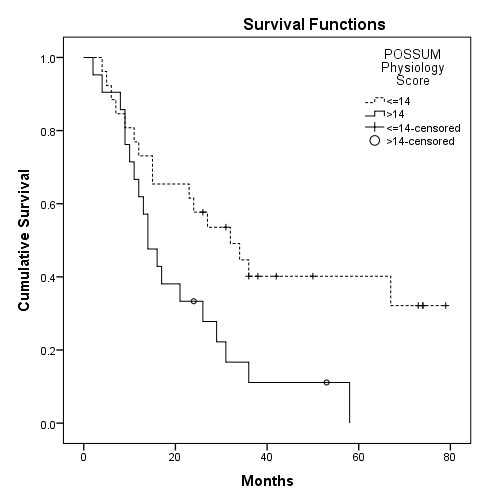
\includegraphics[width=0.8\linewidth]{Figures/cpet_survival_km_possum}
	\caption{Kaplan-Meier Survival Analysis of POSSUM Physiology Score ($\leq14$ vs. $>14$)}
	\label{fig:cpet_survival_km_possum}
\end{figure}

%Create a table looking at means of cardiopulmonary exercise test parameters in survivors vs. non-survivors at 6 months, 1 year and 2 years. This should give three tables as below.

Cardiopulmonary exercise testing parameters in survivors and non-survivors at 6 months, 12 months and 24 months are shown in tables \ref{table:cpet_survival_6months}, \ref{table:cpet_survival_12months}, \ref{table:cpet_survival_24months}. Load achieved at peak exercise was significantly higher in patients who survived at least 6 months (118.5 vs. 76.5 watts, p = 0.026) However, there was no association between any of the other cardiopulmonary exercise testing parameters and survival at 6 months, 12 months or 24 months.

%26/06/15 - fixed all numbers and title
\begin{sidewaystable}[p]
	\centering
	\caption{Preoperative cardiopulmonary exercise test parameters in survivors vs. non-survivors at \textbf{6 months} after curative surgery for ductal adenocarcinoma of the head of the pancreas. (n=47)}
	\label{table:cpet_survival_6months}
	\renewcommand{\arraystretch}{1.2} %Increases space between rows
	\setlength{\tabcolsep}{9pt} %sets the space between columns
	\begin{tabular}{|l | c c c | c c c|}
		\hline
		                             &     \multicolumn{3}{c|}{Anaerobic Threshold}     &       \multicolumn{3}{c|}{Peak Exercise}        \\
		                             & Survivor           & Non-survivor       & $p^*$ & Survivor           & Non-survivor       & $p^*$ \\ \hline
		Load                         & 57 (41 - 67)       & 38 (27 - 54)       & 0.137 & 119 (105 - 130)    & 77 (58 - 100)      & 0.026 \\
		$\dot{V}_E$                  & 21 (20 - 22)       & 23 (19 - 29)       & 0.560 & 52 (45 - 61)       & 49 (38 - 67)       & 0.749 \\
		$\dot{V}_T$                  & 1.0 (1.0 - 1.1)    & 1.1 (0.9 - 1.4)    & 0.721 & 1.9 (1.7 - 1.9)    & 1.6 (1.3 - 2.3)    & 0.560 \\
		$\dot{V}_{O_2}$              & 0.7 (0.7 - 0.7)    & 0.7 (0.6 - 0.9)    & 1.00  & 1.2 (1.2 - 1.3)    & 1.1 (0.8 - 1.4)    & 0.462 \\
		$\dot{V}_{O_2}$/kg           & 8.9 (7.7 - 10.1)   & 10.2 (8.5 - 11)    & 0.173 & 15.8 (13.4 - 18.0) & 15.3 (13.0 - 17.9) & 0.985 \\
		$\dot{V}_E$/$\dot{V}_{O_2}$  & 27.4 (25.3 - 29.2) & 29.8 (27.2 - 31.9) & 0.214 & 44.6 (37.9 - 47.2) & 44.9 (39.8 - 50.2) & 0.560 \\
		$\dot{V}_{CO_2}$             & 0.7 (0.6 - 0.8)    & 0.7 (0.5 - 1.0)    & 0.955 & 1.7 (1.4 - 1.9)    & 1.4 (1.0 - 1.9)    & 0.354 \\
		$\dot{V}_E$/$\dot{V}_{CO_2}$ & 27.7 (26.4 - 29.2) & 30.7 (28.9 - 32.7) & 0.063 & 31.6 (28.3 - 35.6) & 33.8 (31.2 - 37.8) & 0.214 \\
		RER                          & 1.0 (0.9 - 1.0)    & 1.0  (0.9 - 1.1)   & 0.778 & 1.3 (1.2 - 1.5)    & 1.3 (1.2 - 1.4)    & 0.693 \\
		$PET_{O_2}$                  & 108 (105 - 113)    & 113 (108 - 115)    & 0.334 & 124 (119 - 127)    & 125 (121 - 128)    & 0.778 \\
		$PET_{CO_2}$                 & 38 (35 - 40)       & 35 (32 - 37)       & 0.186 & 36 (31 - 40)       & 33 (30 - 36)       & 0.395 \\
		$O_2$Pulse                   & 7.3 (6.0 - 7.8)    & 7.0 (6.0 - 8.0)    & 0.955 & 11.0 (8.7 - 12.9)  & 10.6 (8.6 - 13.1)  & 0.985 \\
		HR                           & 95 (90 - 119)      & 113 (89 - 121)     & 0.778 & 136 (132 - 152)    & 134 (117 - 153)    & 0.693 \\
		Bf                           & 21 (19 - 22)       & 22 (19 - 25)       & 0.486 & 31 (26 - 36)       & 31 (28 - 35)       & 0.749 \\ \hline
	\end{tabular}
	
	All values are median (inter-quartile range). \textit{* p} - Mann-Whitney U test.
\end{sidewaystable}


%26/06/15 - fixed all numbers and title
\begin{sidewaystable}[p]
	\centering
	\caption{Preoperative cardiopulmonary exercise test parameters in survivors vs. non-survivors at 12 months after curative surgery for ductal adenocarcinoma of the head of the pancreas. (n=47) }
	\label{table:cpet_survival_12months}
	\renewcommand{\arraystretch}{1.2} %Increases space between rows
	\setlength{\tabcolsep}{9pt} %sets the space between columns
	\begin{tabular}{|l | c c c | c c c|}
		\hline
		                             &   \multicolumn{3}{c|}{Anaerobic Threshold}    &      \multicolumn{3}{c|}{Peak Exercise}       \\
		                             & Survivor          & Non-survivor      & $p^*$ & Survivor          & Non-survivor      & $p^*$ \\ \hline
		Load                         & 41(33 - 55)       & 38(27 - 54)       & 0.617 & 88(68 - 102)      & 80(58 - 103)      & 0.643 \\
		$\dot{V}_E$                  & 24(21 - 28)       & 21(19 - 29)       & 0.687 & 49(41 - 66)       & 49(38 - 67)       & 0.723 \\
		$\dot{V}_T$                  & 1.1(1.0 - 1.1)    & 1.1(0.8 - 1.5)    & 0.502 & 1.9(1.6 - 1.9)    & 1.6(1.3 - 2.3)    & 0.591 \\
		$\dot{V}_{O_2}$              & 0.7(0.7 - 0.8)    & 0.7(0.6 - 0.9)    & 0.526 & 1.3(1.0 - 1.3)    & 1.1(.8 - 1.4)     & 0.288 \\
		$\dot{V}_{O_2}$/kg           & 9.8(9.4 - 10.9)   & 10.0(8.5 - 11.0)  & 0.661 & 14.6(13.5 - 17.2) & 15.5(13.0 - 17.9) & 0.864 \\
		$\dot{V}_E$/$\dot{V}_{O_2}$  & 30.1(27.1 - 31.3) & 29.7(27.2 - 31.8) & 0.678 & 44.2(39.8 - 48.0) & 45.6(40.2 - 50.2) & 0.414 \\
		$\dot{V}_{CO_2}$             & 0.7(0.6 - 0.8)    & 0.7(0.5 - 1.0)    & 0.733 & 1.5(1.3 - 1.8)    & 1.3(1.0 - 1.9)    & 0.558 \\
		$\dot{V}_E$/$\dot{V}_{CO_2}$ & 29.7(28.7 - 32.1) & 30.3(28.4 - 32.7) & 0.760 & 34.2(32 - 37)     & 33.5(31.2 - 37.4) & 0.836 \\
		RER                          & 1.0(0.9 - 1.0)    & 1.0(0.9 - 1.1)    & 0.386 & 1.3(1.2 - 1.4)    & 1.3(1.3 - 1.4)    & 0.335 \\
		PET$O_2$                     & 113(107 - 114)    & 113(108 - 115)    & 0.651 & 125(120 - 126)    & 125(121 - 128)    & 0.425 \\
		PET$CO_2$                    & 35(34 - 37)       & 35(32 - 38)       & 0.696 & 33(30 - 38)       & 33(30 - 36)       & 0.713 \\
		$O_2$Pulse                   & 7.0(6.7 - 8.0)    & 7.0(6.0 - 8.0)    & 0.835 & 11.1(9.0 - 12.4)  & 10.4(8.6 - 13.1)  & 0.583 \\
		HR                           & 112.3(91 - 128)   & 109(89 - 120)     & 0.421 & 135(128 - 142)    & 133(118 - 159)    & 0.942 \\
		Bf                           & 22(20 - 25)       & 20.5(19 - 24)     & 0.372 & 31(28 - 32)       & 31(28 - 36)       & 0.364 \\ \hline
	\end{tabular}
		
	All values are median (inter-quartile range). \textit{* p} - Mann-Whitney U test.
\end{sidewaystable}
%26/06/15 - fixed all numbers and title
\begin{sidewaystable}[p]
	\centering
	\caption{Preoperative cardiopulmonary exercise test parameters in survivors vs. non-survivors at \textbf{24 months} after curative surgery for ductal adenocarcinoma of the head of the pancreas. (n=47) }
	\label{table:cpet_survival_24months}
	\renewcommand{\arraystretch}{1.2} %Increases space between rows
	%\setlength{\tabcolsep}{9pt} %sets the space between columns
	\begin{tabular}{l | c c c | c c c}
		                             &    \multicolumn{3}{c}{Anaerobic Threshold}    &       \multicolumn{3}{c}{Peak Exercise}       \\
		                             & Survivor          & Non-survivor      & $p^*$ & Survivor          & Non-survivor      & $p^*$ \\ \hline
		Load                         & 43(30 - 58)       & 36(25 - 49)       & 0.475 & 87(67 - 105)      & 82(53 - 103)      & 0.475 \\
		$\dot{V}_E$                  & 24(20 - 30)       & 21(18 - 26)       & 0.239 & 49(40 - 62)       & 49(34 - 67)       & 0.652 \\
		$\dot{V}_T$                  & 1.1(1.0 - 1.2)    & 1.0(0.7 - 1.4)    & 0.361 & 1.8(1.5 - 2.0)    & 1.5(1.1 - 2.4)    & 0.253 \\
		$\dot{V}_{O_2}$              & 0.7(0.6 - 0.8)    & 0.6(0.6 - 0.9)    & 0.379 & 1.2(1.0 - 1.3)    & 1.1(0.8 - 1.5)    & 0.509 \\
		$\dot{V}_{O_2}$/kg           & 10.4(9.0 - 11.2)  & 9.8(8.2 - 10.8)   & 0.312 & 15.6(13.3 - 18.3) & 14.9(12.7 - 17.9) & 0.692 \\
		$\dot{V}_E$/$\dot{V}_{O_2}$  & 30.1(26.8 - 32.5) & 29.5(27.3 - 31.7) & 0.947 & 45.8(39.9 - 49.1) & 44.3(39.5 - 50.2) & 0.904 \\
		$\dot{V}_{CO_2}$             & 0.7(0.6 - 0.9)    & 0.6(0.5 - 1.0)    & 0.397 & 1.4(1.1 - 1.8)    & 1.3(1.0 - 1.9)    & 0.628 \\
		$\dot{V}_E$/$\dot{V}_{CO_2}$ & 30.0(28.6 - 32.2) & 30.4(28.1 - 32.7) & 0.965 & 34.2(31.4 - 37.8) & 33.4(30.8 - 37.4) & 0.878 \\
		RER                          & 1.0(0.9 - 1.1)    & 1.0(0.9 - 1.1)    & 0.750 & 1.3(1.2 - 1.4)    & 1.3(1.3 - 1.4)    & 0.545 \\
		PET$O_2$                     & 113(107 - 115)    & 113(110 - 114)    & 0.741 & 125(121 - 127)    & 125(121 - 128)    & 0.446 \\
		PET$CO_2$                    & 35(33 - 37)       & 35(32 - 38)       & 0.758 & 33(30 - 37)       & 34(31 - 37)       & 0.834 \\
		$O_2$Pulse                   & 7.0(6.0 - 8.0)    & 7.0(5.0 - 8.0)    & 0.580 & 11.3(9.0 - 13.7)  & 10.0(8.0 - 11.8)  & 0.124 \\
		HR                           & 111(92 - 125)     & 111(84 - 120)     & 0.598 & 135(117 - 147)    & 134(123 - 159)    & 0.800 \\
		Bf                           & 21(19 - 24)       & 22(18 - 25)       & 0.808 & 31(28 - 33)       & 33(27 - 36)       & 0.377 \\ \hline
	\end{tabular}
	
	
	All values are median (inter-quartile range). \textit{* p} - Mann-Whitney U test.
\end{sidewaystable}









%Compare significant preoperative factors with tumour factors

\section{Discussion}

 This is considerably less than other common cancers such as colorectal cancer or breast cancer where 5-year survivals across all stages are 60\% and 90\% respectively. However, only 10-20\% of pancreatic cancers are suitable for potentially curative surgery and of patients who undergo curative surgery 5-year survival remains low at approximately 20\%.\parencite{cancerresearchuk_cancer_2014}